\documentclass{standalone}
\usepackage{tikz}
\begin{document}
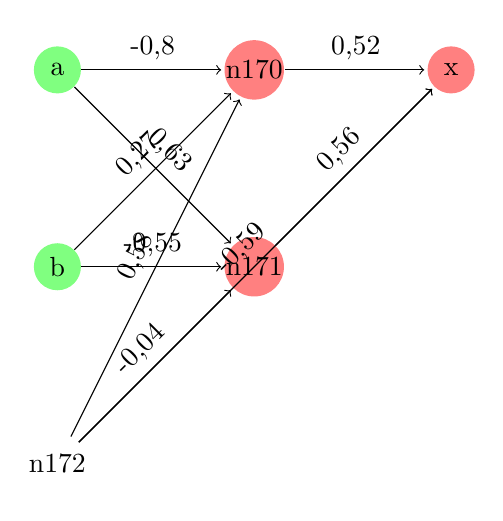
\begin{tikzpicture}[shorten >=1pt,->,draw=black!,node distance=2.5cm]
\tikzstyle{neuron}=[circle,fill=black!25,minimum size=17pt,inner sep=0pt]
\tikzstyle{constant}=[neuron, fill=white!50];
\tikzstyle{sigmoid}=[neuron, fill=red!50];
\tikzstyle{identity}=[neuron, fill=green!50];
\node [identity] (a) {a};
\node [identity,below of=a] (b) {b};
\node [constant,below of=b] (n172) {n172};
\node [sigmoid,right of=a] (n170) {n170};
\node [sigmoid,below of=n170] (n171) {n171};
\node [sigmoid,right of=n170] (x) {x};
\path[every node/.style={sloped,anchor=south,auto=false}]
(n170) edge node {0,52} (x)
(n171) edge node {0,56} (x)
(n172) edge node {-0,04} (n171)
(n172) edge node {0,58} (n170)
(n172) edge node {-0,59} (x)
(a) edge node {0,63} (n171)
(a) edge node {-0,8} (n170)
(b) edge node {0,27} (n170)
(b) edge node {-0,55} (n171)
;\end{tikzpicture}
\end{document}